\section{Results}
\numberwithin{equation}{section}

\subsection{Simulation data}
For the sections \nameref{subsec:validation} and \nameref{subsec:benchmarking},
the simulation was changed to a flat cylindrical gain medium 
(Figure \ref{graphic:samples_round}) to be able to compare the simulation
results with real world experiments. The gain medium has the following
properties:
\\
\\ 
\begin{tabular}{| l | l |}
\hline
Points per plane        & 421\\
\hline
Sample points           & 4210\\
\hline
Planes                  & 10\\
\hline
Triangles               & 812\\
\hline
Prisms                  & 7308\\
\hline
Height                  & 0.7 cm\\
\hline
Diameter                & 6 cm\\
\hline
Material                & $\text{Yb}^{3+}$:YAG ceramic\\
\hline
$\text{Yb}^{3+}$ doping & $2at.\%$\\
\hline
Cladding                & $\text{Cr}^{4+}$:YAG\\
\hline
$\text{Cr}^{4+}$ doping & $0.25at.\%$\\
\hline
Spectrum                & Polychromatic (see Figure \ref{plot:polychromatic_spectrum})\\
\hline
\end{tabular}

\begin{figure}[H]
  \centerline{
    \resizebox{0.5\textwidth} {!} {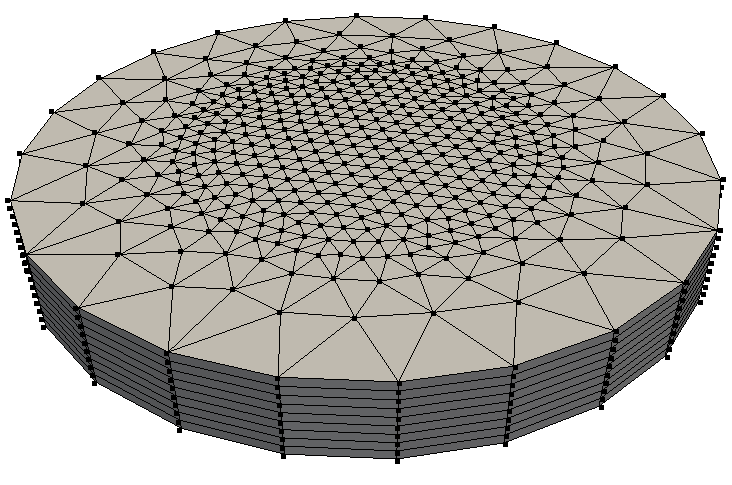
\includegraphics{graphics/samples_round.png}}
  }
  \caption{non-uniform sampling of round active gain medium}
  \label{graphic:samples_round}
\end{figure}

\begin{figure}[H]
  \centerline{
    \resizebox{0.5\textwidth} {!} {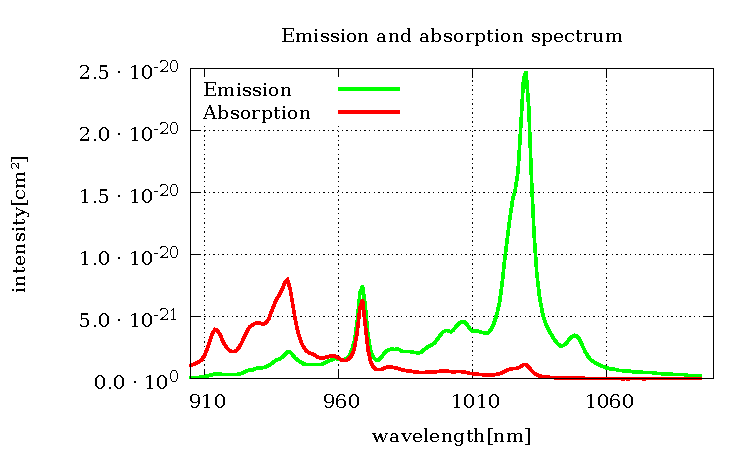
\includegraphics{plot/sigma.pdf}}
  }
  \caption{polychromatic spectrum}
  \label{plot:polychromatic_spectrum}
\end{figure}

\subsection{Setup of the testing environment}
\label{subsec:testingEnvironment}

The benchmarks were conducted on a GPU cluster consisting of 12 compute nodes,
each equipped with a quad core Intel Xeon CPU E5-2609 CPU (2.40GHz), 64GB RAM
and 4 NVIDIA Tesla K20M GPUs with 5GB GDDR5 RAM. Each GPU contains 2496 CUDA cores with a total
peak performance of 3520 GFLOP/s. Job submission is handled by TORQUE\cite{torque} 
with Maui\cite{maui} as scheduling backend. 

% Allready explained in simulation data section
%The modeled gain medium is a
%\textbf{TODO: Daniel should check/complete the description of the medium} YAG
%crystal with a square surface of $16cm^2$\textbf{(?)} and a thickness of
%$0.7cm$\textbf{(?)}. Its upper surface was sampled with 321 points, resulting in
%600 Delaunay triangles (see section \ref{subsec:meshSampling}). The mesh is
%extruded 9 times on the vertical axis, amounting to a total of 3210 sample
%points and 5400 prisms respectively.

\subsection{Validation}
\label{subsec:validation}
We compare the small signal gain at $1030 nm$
derived by the simulation and the results from an experimental setup described in REF. 
It is especially interesting to take a look on the impact of the reflections as well as the polychromatic
approach in our model compared to experimental results. Figure \ref{plot:benchmark} shows
varying simulation configurations and their influence on the
gain development over time compared to an experimentally found gain measurement. Note that the plotted values are discrete and just connected with lines to guide the eye.

\begin{figure}[H]
  \centerline{
    \resizebox{0.5\textwidth}{!}{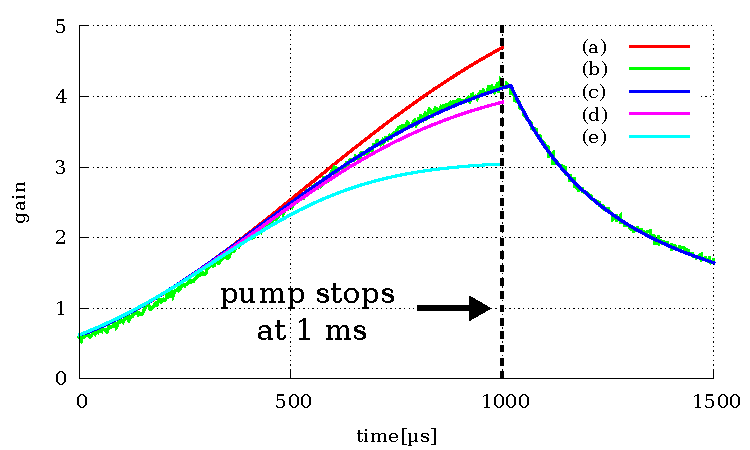
\includegraphics{graphics/benchmark.pdf}}}
  \caption{Simulation compared to measurements:
    (a) polychromatic, no reflections
    (b) experimental measurement
    (c) polychromatic, with reflections
    (d) monochromatic, no reflections
    (e) monochromatic, with reflections}
  \label{plot:benchmark}
\end{figure}

Interestingly, monochromatic simulations without reflections show in this particular case very similar, but smaller, gain values when compared to the full case. Adding reflections overestimates the ASE impact in the monochromatic case and consequently shows a too small gain value. This is mainly attributed to reflected ray paths that are in average longer, especially due to total internal reflection, and consequently reduce the stored energy from the gain medium more severely. 
Simulating only with a polychromatic spectrum overestimates the
gain value on the other hand. As the average emission intensity is lower than the peak
value at $1030 nm$ (see Figure \ref{plot:polychromatic_spectrum}), 
the reduced ASE flux leads to a higher gain.

Consequently a simulation configuration with reflection and polychromatic spectrum enabled 
matches the measured values within the measurement uncertainty and validates our simulation approach.

For the same simulation Figure \ref{graphic:benchmark_4_timeslices} shows five distinct timesteps.
Using \eqref{eq:phi_ase_daniel} and \eqref{eq:gain_local}, it illustrates ${\frac{dn}{dt}|}_{ASE}$ in the sliced gain medium with:

\begin{equation}
  \label{eq:dndt}
  \frac{dn}{dt}\bigg|_{ASE} = \int g_0(\lambda) \cdot \Phi_{ASE}(\lambda)~d\lambda
\end{equation}
\begin{figure}[H]
  \centerline{
    \resizebox{0.5\textwidth}{!}{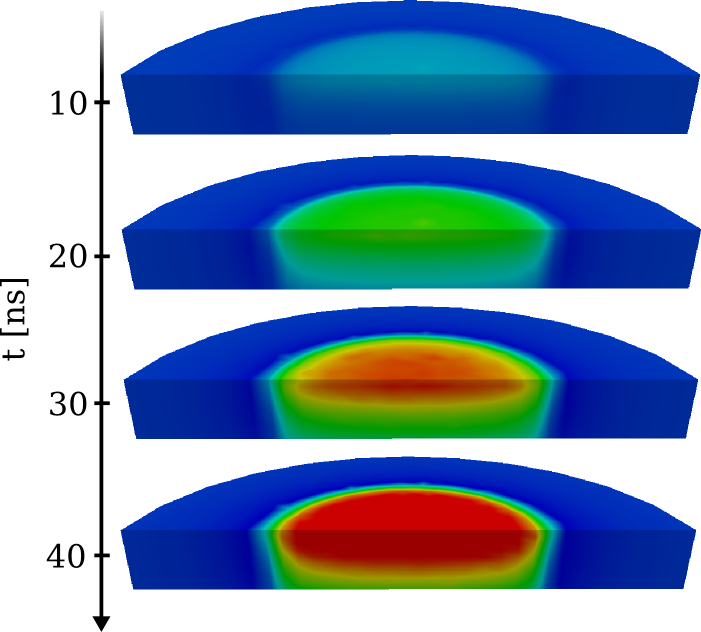
\includegraphics{graphics/benchmark_4_timeslices.png}}}
  \caption{sliced gain medium in 5 timessteps}
  \label{graphic:benchmark_4_timeslices}
\end{figure}

\subsection{Benchmarking}
\label{subsec:benchmarking}
In Figure \ref{plot:runtime}, the runtimes of the original single threaded
algorithm from \cite{ASE2010} are compared to the developed non-adaptive
parallel ASE-flux algorithm with varying numbers of rays to demonstrate
scaling for different workloads. All simulations were done without
reflections to ensure comparability. To increase the number of GPUs, MPI\cite{MPI} was used to distribute the
sample points to all available devices. A sequential overhead for device
allocation 
on the nodes and not fully occupied GPUs are the reasons for the lack of runtime
improvement for low workloads with a small number of rays.

%reflections. To increase the number of GPUs to 48, an \emph{array job} was
%scheduled and the sampling points distributed evenly to the 12 Nodes (each
%hosting 4 GPUs) as seen in section \ref{subsubsec:multigpu}. When using the CPU
%or up to 4 GPUs, the computation uses only a single node, which results in a
%linear scaling of the algorithm. If the cluster's job submission system is used,
%a significant runtime overhead can be seen as a result of the job scheduler
%taking several seconds to process a single job. Therefore, using a high number
%of GPUs can lead to suboptimal performance in otherwise fast computations.
%However, this becomes neglegible for very work intensive simulations.
%\begin{figure}[H]
%  \centerline{
%    \resizebox{0.5\textwidth}{!}{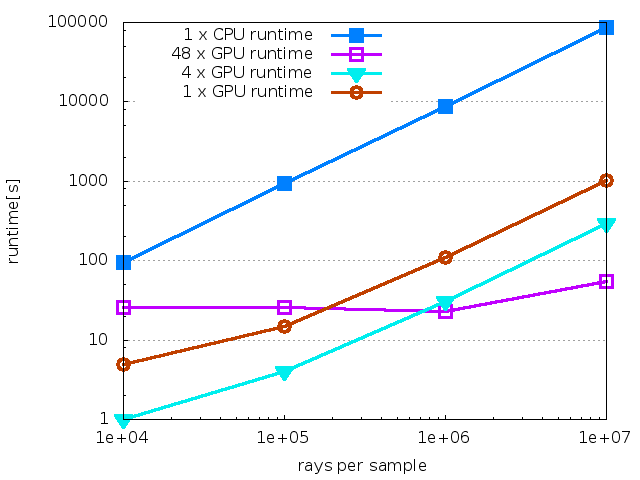
\includegraphics{plot/runtime.png}}}
%  \caption{runtime of sequential algorithm compared to parallel algorithm}
%  \label{plot:runtime}
%\end{figure}

\begin{figure}[H]
  \centerline{
    \resizebox{0.5\textwidth}{!}{
      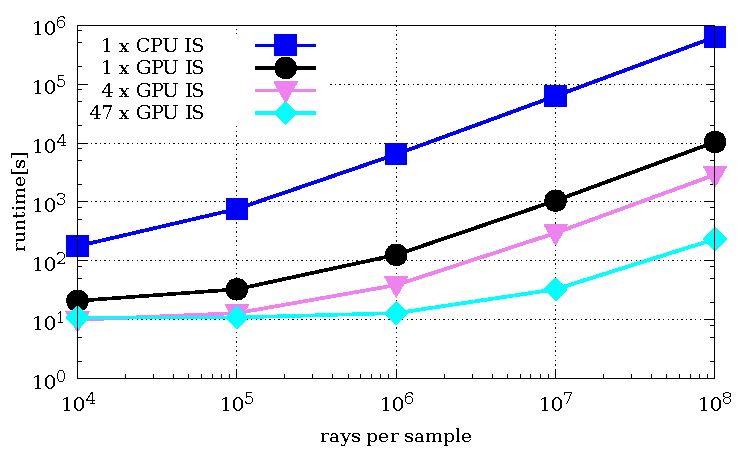
\includegraphics{plot/runtime.pdf}
    }
  }
  \caption{runtime of sequential algorithm compared to parallel algorithm}
  \label{plot:runtime}
\end{figure}

Adaptive sampling usually does not only eliminate outliers, but even reduce the
needed time to do so: By using the idea of a pre-defined $MSE$-threshold, the
precision of the simulation can be adjusted in terms of this threshold rather than
simply increasing the number of rays for all the sample points. Since only a
small subset of sample points actually needs to be sampled with a high
resolution, a small increase in runtime can be sufficient to lower the maximal
$MSE$ values below the desired threshold (Figure \ref{plot:adaptive_runtime}).
This can be adjusted to yield similar simulation results as the non-adaptive
implementation at a fraction of its runtime. Note that some values in the
graphic actually display almost the same runtime, since the computation always
succeeded to stay below the given threshold with very little additional effort.
This is indicated by the black rectangle in Figure \ref{plot:adaptive_runtime}.
\begin{figure}[H]
  \centerline{
    \resizebox{0.5\textwidth}{!}{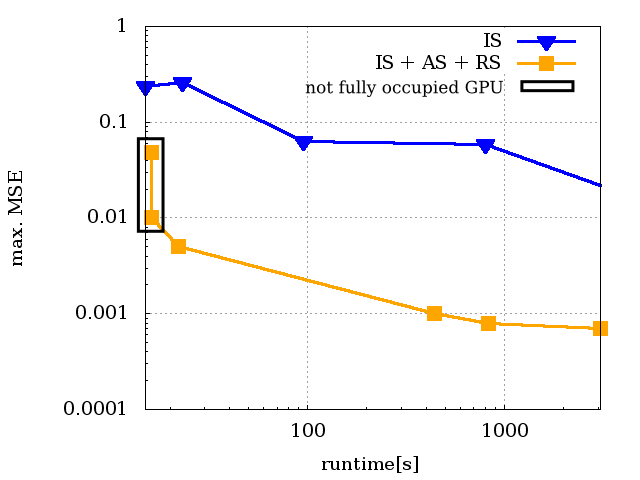
\includegraphics{graphics/adaptive_runtime.png}}}
  \caption{MSE comparision for equal runtimes}
  \label{plot:adaptive_runtime}
\end{figure}

For the adaptive algorithm, simulation times of different sample points can vary
significantly (see Section \ref{subsec:adaptive_sampling}). Therefore, a uniform
partitioning of the sample points among the nodes would result in an unbalanced
workload and reduced efficency for the whole computation. Instead, one of the
nodes acts as a \emph{head node} and manages workload distribution based on demand: As
soon as one of the \emph{compute nodes} is idle, it will request more data to
simulate (Section \ref{subsubsec:multigpu}).
Apart from a constant initialization overhead of 5s, distributing the computation to
multiple devices scales well with all presented methods. (Figure
\ref{plot:gpu_scaling}).
\begin{figure}[H]
  \centerline{
    \resizebox{0.5\textwidth}{!}{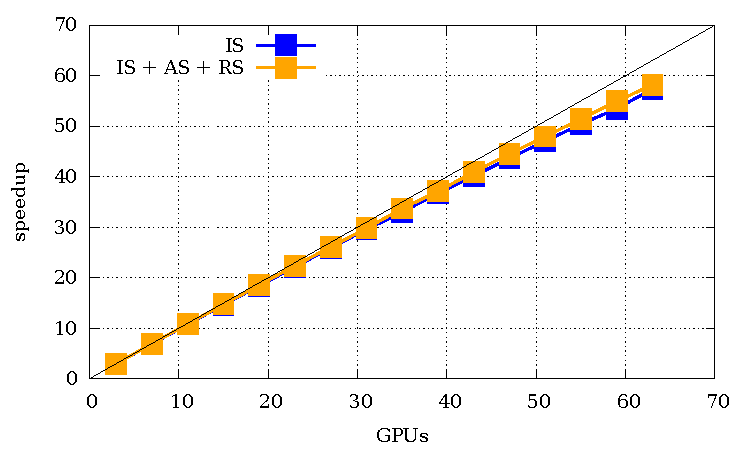
\includegraphics{plot/scaling.pdf}}}
  \caption{speedup on multiple devices}
  \label{plot:gpu_scaling}
\end{figure}

\subsection{Conclusion}
\label{subsec:conclusion}
This paper presented a fast and very scalable implementation of a simulation to
estimate ASE flux in an active gain medium. It seeks to improve the work of
laser physicists by enabling them to properly simulate the described effects
with high speed and high resolution. Experimental details like cladding, surface
coating, refractivites, polychromatic laser pulses and reflections on the upper
and lower side can be modeled and simulated with various additional parameters.

Future improvements could address reflections on the lateral sides of the gain
medium. Also, it will be helpful to further increase the maximum number of rays
(currently there is a maximum of $5\cdot10^8$ rays per sample point). For
example, this could be done rather easily by splitting the simulated rays in
groups and calculating these groups iteratively, combining the results
afterwards.


%Future work should address reflections on the lateral sides of the gain medium
%to allow the simulation of lateral feedback. The current implementation only
%supports reflections on the upper and lower surface. Furthermore, these upper
%and lower surfaces need to be coplanar due to the structure of the mesh
%(Section \ref{subsec:meshSampling}).
%Another limitation originates from the fact that each simulation uses a mapping
%from rays to their respective starting position. For a large number of rays,
%this can lead to a substancial amout of allocated memory. With the current
%hardware (Section \ref{subsec:testingEnvironment}) and implementation, each sample
%point can be simulated with a maximum of $6.5\cdot10^8$ rays. To push this limit
%further, a more sophisticated mapping needs to be implemented. This could
%be done by simply splitting the mapping in different parts and calculating them
%iteratively.
